% 第四章采用大论文的状态编码与三头规则选择框架。
% 英文进入正文；中文仅作核对与待补充说明，不参与排版。
\section{Dynamic Heterogeneous Graph-based Rule Selection}
\label{sec:method}

Dynamic processing--assembly scheduling requires a policy to distinguish changes in operation progress,
resource availability, and assembly readiness. These changes have different implications for routing,
sequencing, and recovery. The method therefore combines a dynamic heterogeneous graph, meta-path
semantic attention, and decision-specific state readout with three PPO rule-selection heads. The
encoder supplies the state information used to select rules, while the environment enforces the
physical constraints in Section~\ref{sec:problem}.

% 方法区分状态构建、语义编码与策略学习。状态编码为规则选择提供信息，
% 环境继续负责第三章定义的物理约束，不把网络输出直接当成可执行安排。

\subsection{Overall Framework}
\label{subsec:framework_overview}

Figure~\ref{fig:framework} outlines the interaction between the environment and the policy. At
decision index $n$, corresponding to physical time $t_n$, the environment supplies the observation
$x_n$, decision type $\vartheta_n\in\{R,S,RE\}$, and feasible object set
$\mathcal D_n^{\vartheta_n}$. The three types denote machine routing, operation sequencing, and
failure recovery. Several decisions may occur at the same physical time because each dispatch changes
the choices available to subsequent dispatches.

% 环境提供状态、决策类型与可行对象集合。R、S、RE分别对应机器分配、
% 工序排序与故障恢复。同一仿真时刻可以连续执行多个决策。

The observation is mapped to a graph $G_n$. A shared HGNN aggregates typed relations and enhances
node representations through attention over processing--assembly meta-paths. Role-based readout
produces a representation for each decision type. Only the corresponding Actor head is activated to
select a rule from its fixed candidate set. The rule scores feasible objects and returns a concrete
decision to the simulator. Trajectory rewards jointly train the encoder, Actor heads, and Critic.

% 共享编码器先聚合异构关系，再进行元路径注意力增强和角色汇聚。
% 对应Actor头选择规则，规则评价可行对象并生成实际调度决策。

\begin{figure*}[t]
 \centering
 \captionsetup{name=Figure}
 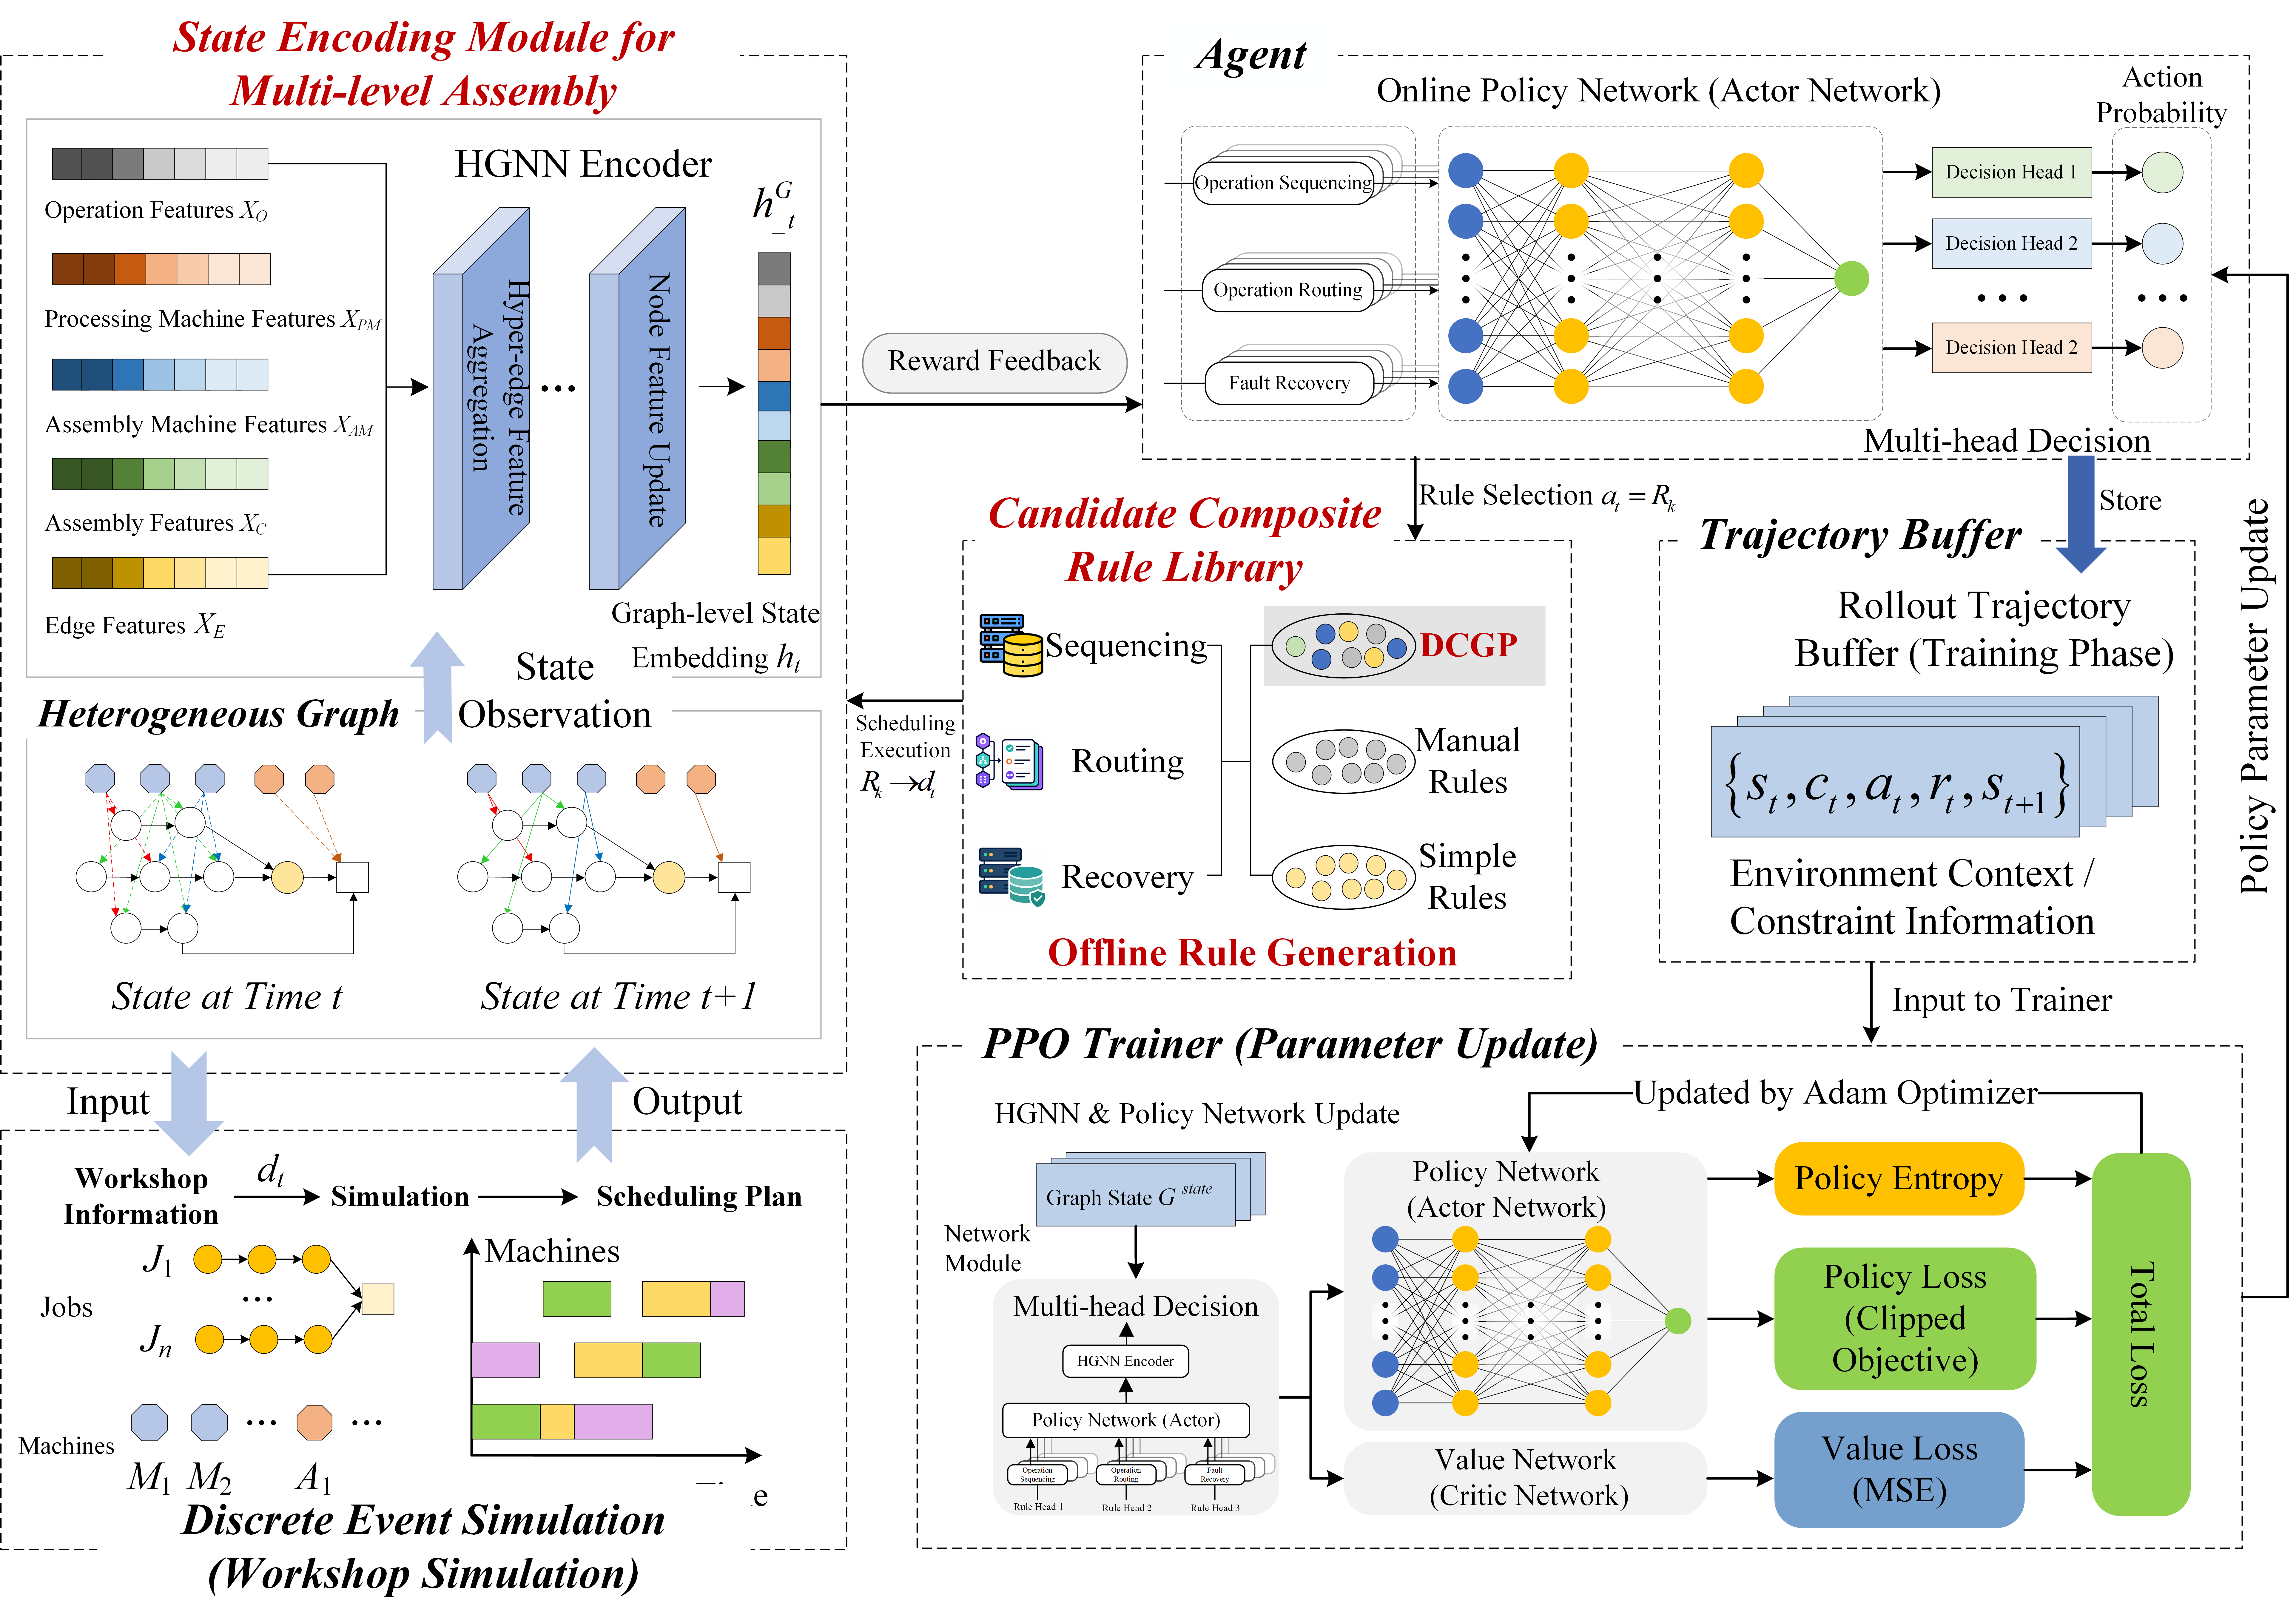
\includegraphics[width=0.95\textwidth]{figures/F2基于规则级决策的反应式调度总体框架.png}
 \caption{Framework of dynamic graph encoding and adaptive dispatching rule selection.}
 \label{fig:framework}
\end{figure*}

A rule action $a_n$ is distinct from the resulting scheduling decision $d_n$. The policy learns which
rule to invoke, rather than directly selecting an operation or machine. Feasibility, including flexible
assembly matching and committed component usage, remains an environment constraint. Candidate rules are
fixed before training and unchanged during evaluation; rule evolution is outside the scope of this
state-encoding method.

% 动作是规则，具体决策是规则调用结果。规则库训练前固定，不展开规则演化。

\subsection{Dynamic Heterogeneous Graph Construction and Update}
\label{subsec:temporal_graph}

\subsubsection{Typed Graph and Observable Features}

The state at decision $n$ is represented as
\begin{equation}
 s_n=(G_n,\boldsymbol{z}_n,\vartheta_n),\qquad
 G_n=(V_n,E_n,\phi,\psi,\boldsymbol{X}_n),
 \label{eq:temporal_graph}
\end{equation}
where $\phi$ and $\psi$ identify node and edge types, $\boldsymbol{X}_n$ contains node features, and
$\boldsymbol{z}_n$ contains observable global statistics. Nodes represent processing operations $O$,
assembly operations $A$, processing and assembly machines $M$, and assembly junctions $S_\ell$.
Start and end nodes delimit the production network. An assembly junction represents a structural
dependency rather than an additional executable task.

% 图中包括加工工序、装配工序、设备和层级装配连接点。
% 起止节点界定生产网络，连接点不额外消耗物理加工资源。

Edges distinguish technological precedence, machine eligibility, active assignments, and assembly
dependencies. Eligibility does not disappear when a machine becomes busy or fails: its current
availability is recorded separately. Undecided assembly matches retain compatible relations, whereas
selected matches are marked as committed. Reverse message-passing relations preserve their semantic
types. This construction retains the flexible matching mechanism of the base problem.

% 候选资格与设备当前可用性分开表示。未确定装配匹配保留兼容关系，
% 实际匹配选定后标记，不提前将所有同类型工件绑定至固定产品。

Operation features describe execution status, release information, current duration estimates,
remaining work, predecessor completion, and baseline deviations. Assembly features describe component
readiness and hierarchy. Machine features describe availability, failure status, occupancy, and load.
An indicator distinguishes operations with baseline records from newly arrived tasks. Global
statistics summarize workload, unfinished tasks, and accumulated deviation. Normalization references
are fixed by the training protocol, without using unrevealed future orders or disturbances.

% 工序、装配与机器分别记录进度、齐套和资源状态；新订单用基准存在标记区分。
% TODO：最终特征清单、缺失值编码和归一化常数须与程序逐项核对。

\subsubsection{Event-driven Graph Update}

The physical transition is defined in Eq.~\eqref{eq:event_decision_transition}; graph updating maps
the resulting state changes into the next observation:
\begin{equation}
 G_{n+1}=\mathcal U_G(G_n,\Delta x_n),
 \label{eq:graph_update}
\end{equation}
where $\Delta x_n$ includes the executed decision and intervening observed events. Assignment activates
an execution relation. Completion releases the machine and updates successor readiness. Failure changes
machine availability and interrupts the affected operation; recovery restores availability. A duration
update revises operation-time and assembly-readiness estimates. An urgent arrival adds its revealed
operations, assembly structure, and machine-eligibility relations.

% 第三章描述物理状态如何变化，本节描述事件如何更新图。
% 完成、故障、恢复、工时波动、插单以及决策执行分别更新相关属性或关系。

Figure~\ref{fig:temporal_graph} illustrates graph evolution during production. Completed nodes may
remain as historical context but cannot be dispatch candidates. Order arrivals can increase graph
size without changing the embedding dimension or the fixed rule-action sets. Dynamic updating here
refers to event-dependent graph structure and features; it does not introduce a recurrent network or
an additional temporal-fusion module.

% 图随插单扩展，编码维数与规则动作数量保持不变。
% 删除原稿额外引入的时序门控，按F3采用当前动态图与执行记录编码。

\begin{figure*}[t]
 \centering
 \captionsetup{name=Figure}
 \includegraphics[width=0.95\textwidth]{figures/F4动态调度过程中的图状态演化.png}
 \caption{Evolution of the heterogeneous scheduling graph during production execution.}
 \label{fig:temporal_graph}
\end{figure*}

\subsection{Meta-path Semantic Attention-based State Encoding}
\label{subsec:hgnn_state}

The encoder in Fig.~\ref{fig:attention_hgnn} distinguishes typed neighborhood aggregation from
semantic fusion. A precedence chain, a shared machine, and an assembly junction convey different
scheduling information even when they connect the same operations. Their representations are therefore
formed separately before attention-based residual enhancement and decision-specific readout.

% 本节是方法重点：关系聚合、元路径语义、注意力残差增强和角色汇聚。

\begin{figure*}[p]
 \centering
 \captionsetup{name=Figure}
 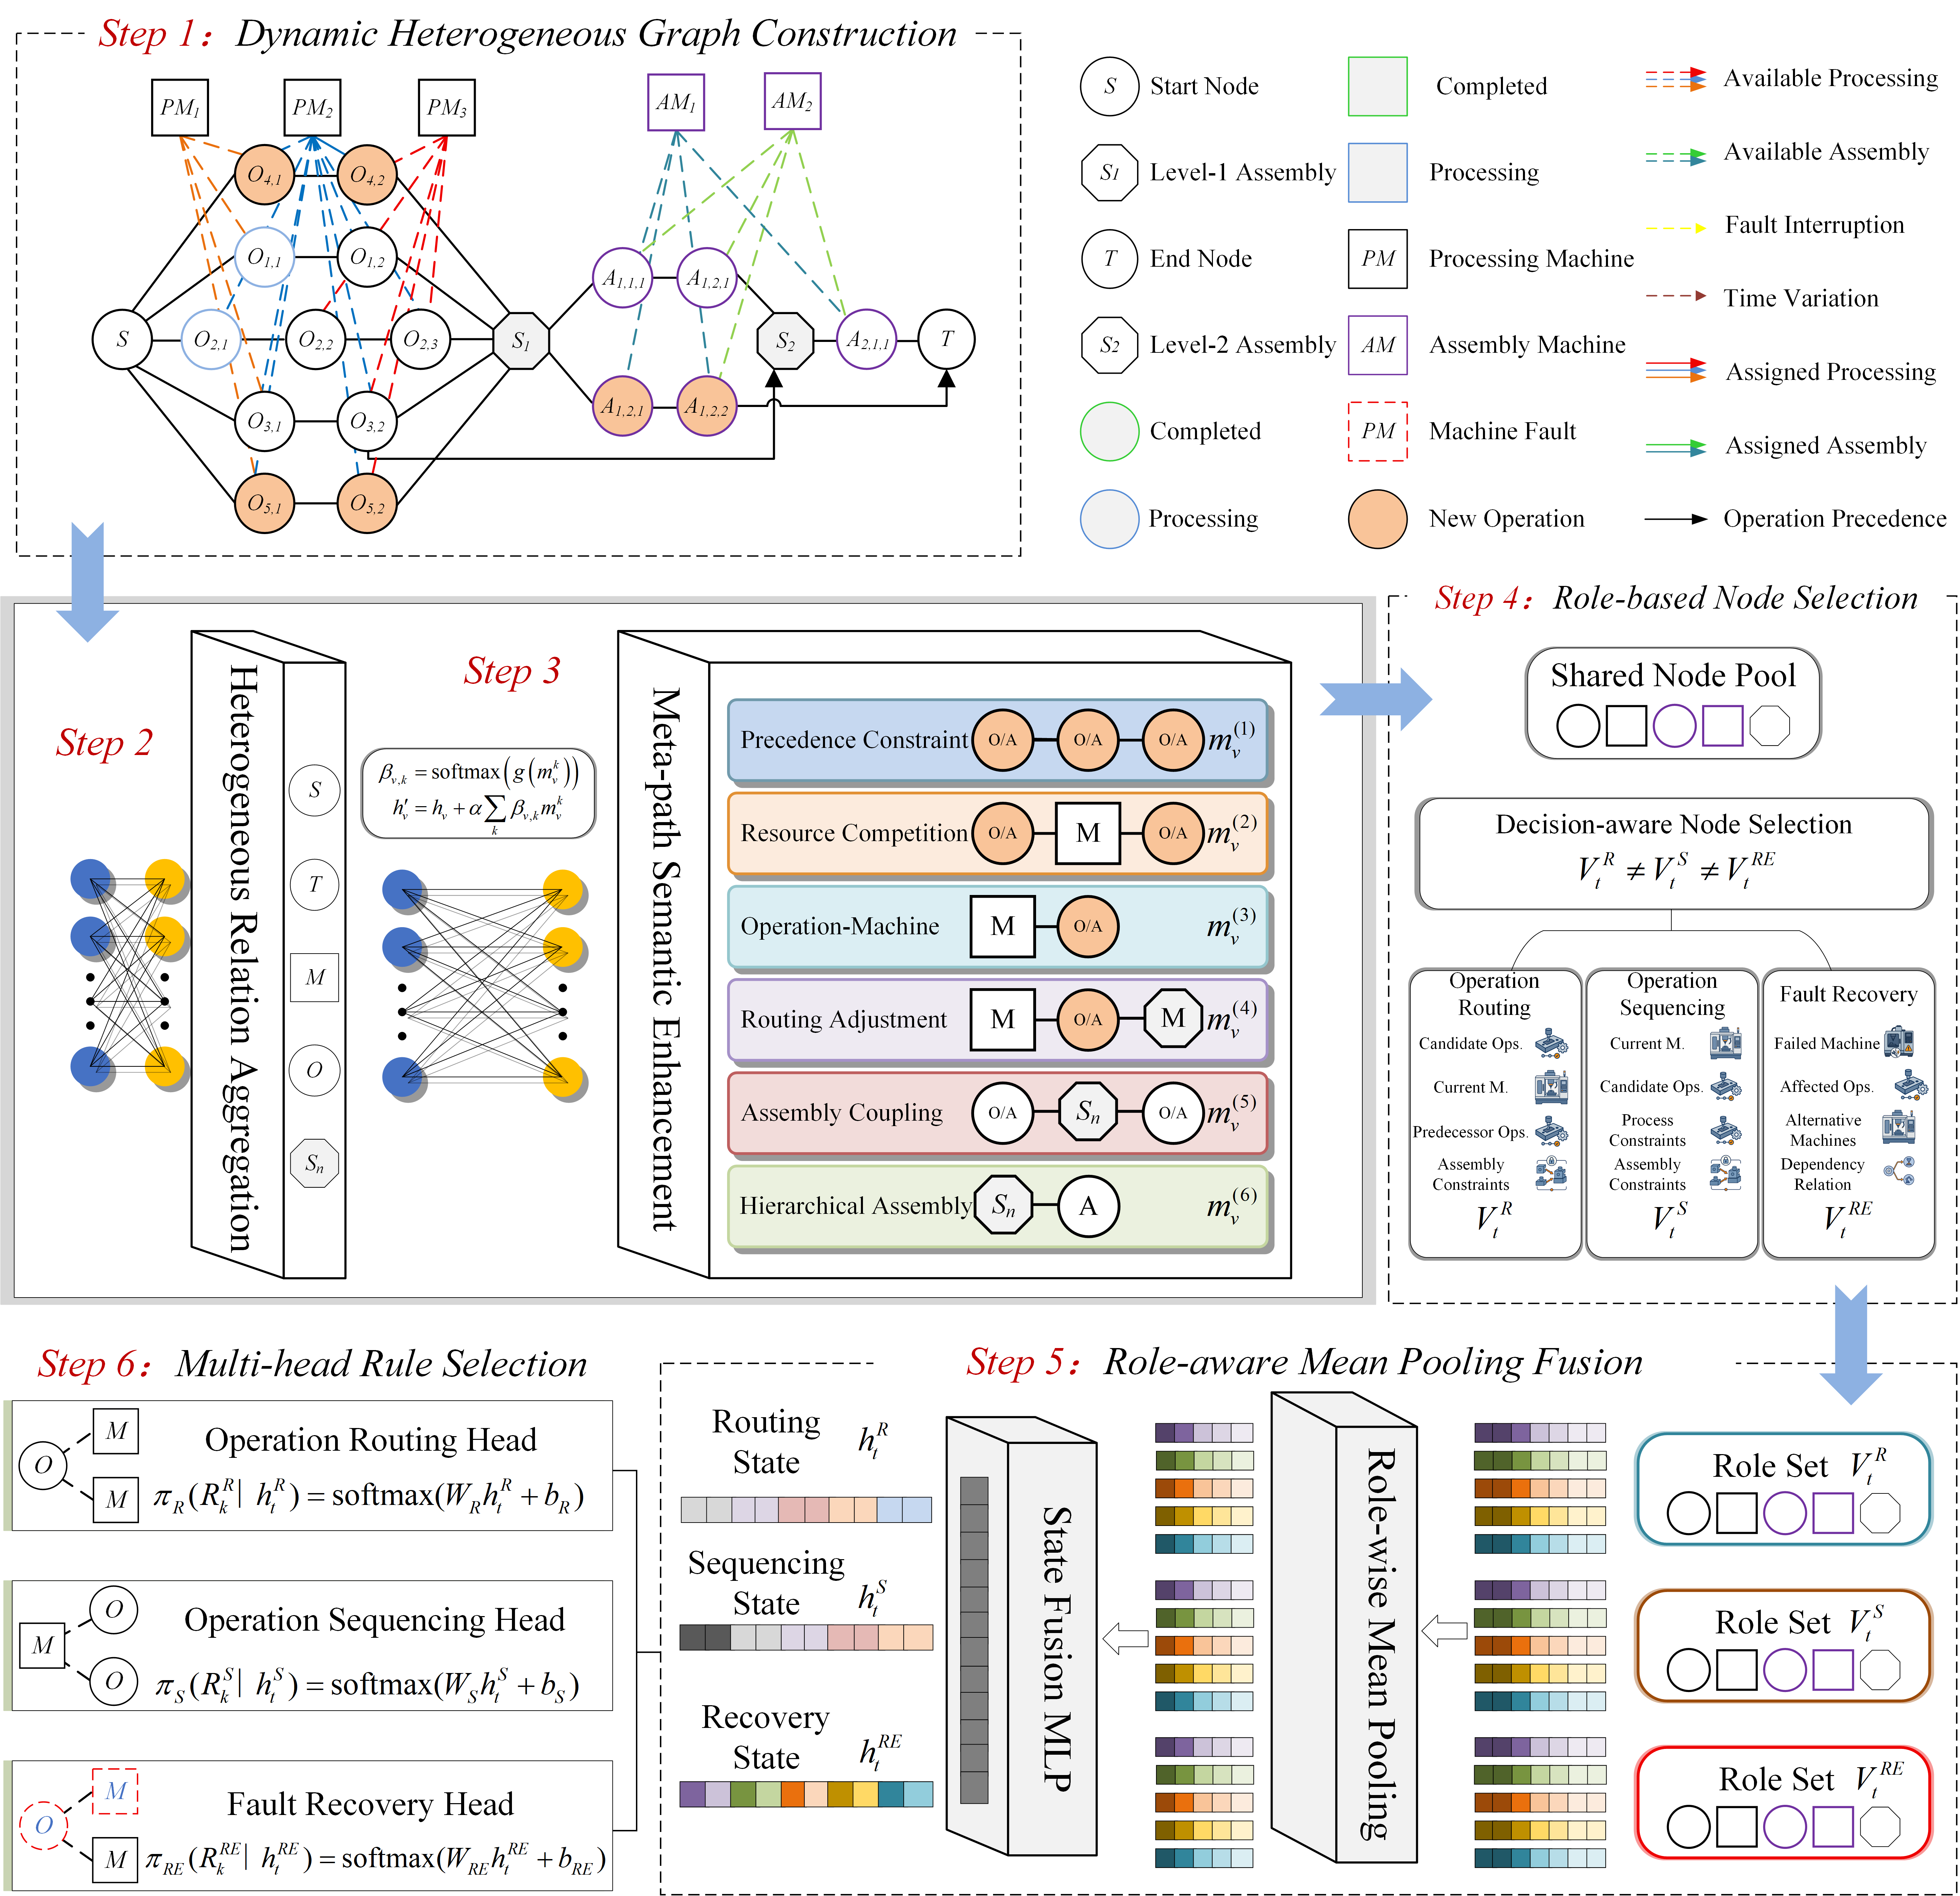
\includegraphics[width=0.98\textwidth,height=0.80\textheight,keepaspectratio]{figures/F3融合装配环境的原路径注意力机制(1).png}
 \caption{Meta-path semantic attention, role-based state readout, and multi-head rule selection.}
 \label{fig:attention_hgnn}
\end{figure*}

\subsubsection{Heterogeneous Relation Aggregation}

Type-specific projections map raw features into a common hidden space:
\begin{equation}
 \boldsymbol{h}^{(0)}_{v,n}
 =\sigma(\boldsymbol{W}_{\phi(v)}\boldsymbol{x}_{v,n}+\boldsymbol{b}_{\phi(v)}).
 \label{eq:type_projection}
\end{equation}
At layer $l$, relation aggregation gives
\begin{equation}
 \boldsymbol{h}^{(l+1)}_{v,n}=\sigma\!\left(
 \boldsymbol{W}_0^{(l)}\boldsymbol{h}^{(l)}_{v,n}
 +\sum_{r\in\mathcal R_G}\sum_{u\in\mathcal N_r(v)}
 \alpha^{(l,r)}_{vu,n}\boldsymbol{W}_r^{(l)}\boldsymbol{h}^{(l)}_{u,n}\right),
 \label{eq:relation_aggregation}
\end{equation}
where $\mathcal N_r(v)$ is the relation-$r$ neighborhood and $\alpha^{(l,r)}_{vu,n}$ denotes
normalized neighbor weights. Each relation has its own mapping, separating machine information from
technological and assembly information. Let $\boldsymbol{h}_{v,n}$ denote the final aggregated embedding.

% 邻居聚合权重与后续语义注意力分属不同层次。
% TODO：核验邻居权重的具体计算、层数、维数及激活函数。

\subsubsection{Processing--Assembly Meta-path Semantics}

Six typed patterns describe complementary scheduling semantics, as listed in
Table~\ref{tab:meta_paths}. Here $O/A$ denotes a processing or assembly operation. The patterns are
computational information paths, not additional physical precedence constraints. For example,
$O/A$--$M$--$O/A$ captures competition through a shared machine, whereas
$O/A$--$S_\ell$--$O/A$ captures coupling through an assembly junction.

% 六类元路径遵循F3，区分工艺、竞争、匹配、路由、装配耦合和层级依赖。

\begin{table}[t]
 \centering
 \captionsetup{name=Table}
 \caption{Meta-path patterns and scheduling semantics.}
 \label{tab:meta_paths}
 \small
 \setlength{\tabcolsep}{3pt}
 \begin{tabular}{@{}c p{0.39\linewidth} p{0.48\linewidth}@{}}
 \toprule
 $k$ & Typed pattern & Scheduling semantics \\
 \midrule
 1 & $O/A$--$O/A$--$O/A$ & Technological and assembly precedence \\
 2 & $O/A$--$M$--$O/A$ & Shared-resource competition \\
 3 & $M$--$O/A$ & Operation--machine association \\
 4 & $M$--$O/A$--$M$ & Routing and reassignment context \\
 5 & $O/A$--$S_\ell$--$O/A$ & Coupling of assembly branches \\
 6 & $S_\ell$--$A$ & Hierarchical assembly dependency \\
 \bottomrule
 \end{tabular}
\end{table}

Let $\mathcal I_k(v,n)$ contain valid instances of pattern $k$ associated with node $v$, and let
$\mathcal N_k(v,n)$ contain their participating nodes. The semantic representation is
\begin{equation}
 \boldsymbol{m}^{(k)}_{v,n}=\operatorname{AGG}_k
 \left(\{\boldsymbol{h}_{u,n}\}_{u\in\mathcal N_k(v,n)}\right).
 \label{eq:meta_path_embedding}
\end{equation}
The pattern-specific operator retains semantic identity when aggregating participating nodes.
Absent patterns are excluded from attention normalization. Thus a missing assembly branch or an
inapplicable routing pattern is not interpreted as an informative zero-valued observation.

% AGG是对F3路径聚合模块的接口表达，不虚构尚未核验的具体实现。
% TODO：核验路径实例、方向、重复计数及AGG算子，补齐可复现定义。

\subsubsection{Semantic Attention and Residual Enhancement}

For valid pattern set $\mathcal K_v(n)$, a learnable scoring function $g$ gives
\begin{equation}
 \begin{aligned}
 e_{v,k,n}&=g(\boldsymbol{m}^{(k)}_{v,n}), \\
 \beta_{v,k,n}&=\frac{\exp(e_{v,k,n})}
 {\sum_{j\in\mathcal K_v(n)}\exp(e_{v,j,n})}.
 \end{aligned}
 \label{eq:relation_semantic_attention}
\end{equation}
The enhanced representation follows the residual construction in Fig.~\ref{fig:attention_hgnn}:
\begin{equation}
 \boldsymbol{h}'_{v,n}=\boldsymbol{h}_{v,n}
 +\eta\sum_{k\in\mathcal K_v(n)}\beta_{v,k,n}\boldsymbol{m}^{(k)}_{v,n}.
 \label{eq:hgnn_update}
\end{equation}
Coefficient $\eta$ corresponds to the residual coefficient $\alpha$ in the figure and is distinct
from the neighbor weights in Eq.~\eqref{eq:relation_aggregation}. When no pattern is valid, the
residual contribution is zero. The original node embedding is preserved, while semantic weights
respond to changing operation and resource features. Whether this mechanism improves scheduling,
rather than merely changing the representation, is examined through controlled ablations.

% 注意力在有效路径之间归一化，残差保留原节点表示。
% 不预先宣称故障时某条路径一定获得最高权重，具体作用由消融验证。
% TODO：评分函数g的结构及残差系数的取值方式须与代码核对。

\subsubsection{Decision-specific Role Readout}

Routing uses the current operation, eligible machines, predecessors, and assembly context. Sequencing
uses the current machine, candidate operations, and their precedence and assembly context. Recovery
uses the failed machine, interrupted operation, alternative machines, and dependent tasks. The
corresponding node sets $V_n^R$, $V_n^S$, and $V_n^{RE}$ need not coincide.

% 三类角色集合关注不同决策对象，可以不同，但不要求每次两两不相等。

For role subset $V_{n,c}^{\vartheta}$, role-wise mean pooling and fusion produce
\begin{equation}
 \begin{aligned}
 \boldsymbol{p}_{n,c}^{\vartheta}
 &=\frac{1}{|V_{n,c}^{\vartheta}|}
 \sum_{v\in V_{n,c}^{\vartheta}}\boldsymbol{h}'_{v,n},
 \quad |V_{n,c}^{\vartheta}|>0, \\
 \boldsymbol{h}_n^{\vartheta}
 &=\operatorname{MLP}_{\vartheta}\!\left(
 \mathop{\Vert}_{c\in\mathcal C_{\vartheta}}\boldsymbol{p}_{n,c}^{\vartheta}
 \Vert\boldsymbol{z}_n\right).
 \end{aligned}
 \label{eq:graph_readout}
\end{equation}
An empty role subset is represented by a zero vector with a presence indicator. The readout therefore
has fixed dimension and yields $\boldsymbol{h}_n^R$, $\boldsymbol{h}_n^S$, and $\boldsymbol{h}_n^{RE}$.
This step uses mean pooling, not another attention layer.

% 按角色均值池化后融合为三个状态向量，与F3保持一致。
% TODO：角色类别、空集处理与全局统计量按程序核验。

\subsection{Multi-head PPO-based Adaptive Rule Selection}
\label{subsec:ppo_policy}

\subsubsection{Rule Actions and Scheduling Decisions}

The rule-level decision process is
\begin{equation}
 \mathcal M=\langle\mathcal S,\mathcal U,P,\mathcal R_{\mathrm{rew}},\gamma\rangle,
 \qquad\mathcal U(s_n,\vartheta_n)=\mathcal R^{\vartheta_n},
 \label{eq:mdp}
\end{equation}
where $\mathcal R^R$, $\mathcal R^S$, and $\mathcal R^{RE}$ are fixed routing, sequencing, and
recovery rule sets. Selecting $a_n=R_\nu^{\vartheta_n}$ induces
\begin{equation}
 d_n=\operatorname{Select}_{d\in\mathcal D_n^{\vartheta_n}}
 R_\nu^{\vartheta_n}(d;x_n,S^0).
 \label{eq:rule_decoding}
\end{equation}
Each rule specifies its ranking direction and deterministic tie breaking. An empty object set does
not trigger a rule action. Rules with unavailable inputs require an explicit fallback or applicability
mask; newly arrived orders have no fictitious baseline records. Assembly compatibility and committed
component usage are checked before execution.

% 规则库不是创新点，仅作为固定动作接口。
% TODO：最终规则库尚未确定，补充规则数量、清单、公式、方向及回退。
% 不将讨论中的3/4/3配置或DCGP规则写成已采用事实。
% TODO：明确环境中柔性装配匹配的生成与提交步骤。

The simulator transition includes decoding and execution of the selected rule, followed by intervening
observed events:
\begin{equation}
 s_{n+1}\sim P(\cdot\mid s_n,a_n).
 \label{eq:state_transition}
\end{equation}
The next decision can occur at the same physical time. The transition kernel is induced by the
environment and its fixed decoding conventions rather than learned separately.

% 规则级转移包含解码与执行，同一时刻可以继续触发下一个决策。

\subsubsection{Three Actor Heads and Dual-objective Reward}

Only the Actor head for the current decision type is activated:
\begin{equation}
 \pi_{\vartheta_n}(\cdot\mid s_n)=\operatorname{softmax}\!\left(
 \boldsymbol{W}_{\vartheta_n}\boldsymbol{h}_n^{\vartheta_n}
 +\boldsymbol{b}_{\vartheta_n}+\boldsymbol\mu_n^{\vartheta_n}\right),
 \label{eq:actor_policy}
\end{equation}
where the rule applicability mask is zero for applicable rules and $-\infty$ otherwise. Training
samples from this distribution. The evaluation convention and candidate rules are held fixed when
comparing different selectors.

% 三个Actor头独立输出，编码器共享；掩码针对规则适用性。
% TODO：测试采用最大概率还是采样，按实际实验报告。

Following Section~\ref{subsec:mathematical_model}, feedback combines potential shaping, exception
penalties, and dual-objective terminal evaluation:
\begin{equation}
 \begin{aligned}
 r_n&=\gamma\Phi(s_{n+1})-\Phi(s_n)+r_n^{\mathrm{pen}}+r_n^{\mathrm{term}},
 \\
 r_n^{\mathrm{term}}&=-\alpha_T\frac{D_{\mathrm{dev}}(S,S^0)}{D_{\mathrm{ref}}}
 -\beta_T\frac{C_{\max}(S)}{C_{\mathrm{ref}}}.
 \end{aligned}
 \label{eq:reward}
\end{equation}
The terminal expression in Eq.~\eqref{eq:reward} applies at normal termination and is zero otherwise.
Positive references $D_{\mathrm{ref}}$ and $C_{\mathrm{ref}}$
are fixed independently of test outcomes. Weights $\alpha_T,\beta_T\ge0$ specify the objective
preference. The potential summarizes observable deviation, completion estimates, remaining workload,
load imbalance, assembly blocking, and recovery waiting. Its terminal value is zero. Invalid execution,
deadlock, and simulation failure receive exception penalties rather than normal terminal scores.

% 奖励沿用大论文的塑形、异常惩罚与双目标终端评价结构。
% TODO：完整势函数及异常惩罚数值须按程序补齐，不能用指标罗列代替定义。
% 终态势函数置零，归一化参照不使用测试结果回填。

For trade-off evaluation, different pairs $(\alpha_T,\beta_T)$ are trained independently. Test schedules
from the frozen preference policies are pooled and nondominated schedules retained. Hypervolume and
spread then require common objective normalization and evaluation budgets. One preference policy alone
does not constitute a generated Pareto set.

% 沿用大论文多组偏好独立训练、测试汇总并非支配筛选的路线。
% TODO：权重组、独立运行次数、解集合并方式及HV参考点须核验。

\subsubsection{PPO Optimization and Online Execution}

A Critic $V_\omega(s_n,\vartheta_n)$ estimates the return from shared state information and the current
decision context. Temporal-difference residuals and generalized advantages are
\begin{equation}
 \begin{aligned}
 \delta_n&=r_n+\gamma V_\omega(s_{n+1},\vartheta_{n+1})
 -V_\omega(s_n,\vartheta_n), \\
 \widehat A_n&=\sum_{j=0}^{N-n-1}(\gamma\lambda)^j\delta_{n+j}.
 \end{aligned}
 \label{eq:gae}
\end{equation}
Terminal states have zero bootstrap value, whereas nonterminal rollout truncations retain value
bootstrapping. Here $N$ is the trajectory boundary and $\lambda$ the advantage parameter. Discounting
is defined per decision rather than per unit of physical time.

% 正常终态不自举，非终止截断保留自举。折扣按决策步计，不按物理时间计。

For each stored sample, the likelihood ratio uses its active head:
\begin{equation}
 \rho_n(\theta)=\frac{\pi_{\theta,\vartheta_n}(a_n\mid s_n)}
 {\pi_{\theta_{\mathrm{old}},\vartheta_n}(a_n\mid s_n)}.
 \label{eq:policy_ratio}
\end{equation}
PPO maximizes the clipped objective~\cite{schulman2017ppo}
\begin{equation}
 \begin{aligned}
 \bar\rho_n(\theta)
 &=\operatorname{clip}(\rho_n(\theta),1-\epsilon,1+\epsilon),\\
 L^{\mathrm{clip}}(\theta)
 &=\mathbb E_n\!\left[\min\left\{
 \rho_n(\theta)\widehat A_n,\bar\rho_n(\theta)\widehat A_n\right\}\right],
 \end{aligned}
 \label{eq:ppo_clip}
\end{equation}
with joint minimization loss. Writing $V_n=V_\omega(s_n,\vartheta_n)$ and
$\pi_n=\pi_{\theta,\vartheta_n}(\cdot\mid s_n)$ gives
\begin{equation}
 L=-L^{\mathrm{clip}}+c_V\mathbb E_n[(V_n-\widehat V_n)^2]
 -c_H\mathbb E_n[\mathcal H(\pi_n)].
 \label{eq:ppo_total_loss}
\end{equation}
Here $\widehat V_n$ is the return target, $\epsilon$ is the clipping parameter, and $c_V,c_H\ge0$.
Each sample updates its active head and the shared encoder together with the Critic. Decision types
and applicability masks are stored so the same action distribution is used when recomputing ratios.

% 概率比不在不同头间混算；缓存决策类型、动作与规则掩码。

\begin{algorithm}[t]
\caption{Multi-head rule-selection training}
\label{alg:training}
\small
\begin{algorithmic}[1]
\Require Instances, baselines, scenarios, rules, preferences
\Ensure Trained encoder and preference policies
\For{each objective preference}
 \State Initialize encoder, Actor heads, and Critic
 \For{each rollout}
  \State Reset the instance, baseline, and scenario
  \While{the episode has not terminated}
   \State Process events; obtain $x_n$, $\vartheta_n$, $\mathcal D_n^{\vartheta_n}$
   \If{$\mathcal D_n^{\vartheta_n}=\varnothing$}
    \State Advance events or terminate
   \Else
    \State Update and encode $G_n$
    \State Read out $\boldsymbol{h}_n^{\vartheta_n}$
    \State Sample rule $a_n$ from the active head
    \State Decode and execute decision $d_n$
    \State Store transition, head type, and mask
   \EndIf
  \EndWhile
  \State Compute returns and advantages
  \State Update networks using Eq.~\eqref{eq:ppo_total_loss}
 \EndFor
\EndFor
\end{algorithmic}
\end{algorithm}

Online execution freezes all parameters and candidate rule sets. Each decision updates the graph,
encodes the active role state, selects a rule, and decodes it into a feasible scheduling decision.
No online rule evolution is performed. Comparisons that isolate the encoder or selector use identical
rules, decoding conventions, scenarios, and evaluation budgets.

% 在线固定网络与规则库，只执行图更新、编码、选择和解码。
% TODO：训练超参数、Critic输入、完整规则与势函数、推理耗时待程序核验。
\FloatBarrier
